\documentclass[a4paper,12pt]{article}
\usepackage{anyfontsize}
\usepackage[utf8]{inputenc}
\usepackage[T1, T2A]{fontenc}
\usepackage[english, russian]{babel}
\fontsize{14pt}{16pt}\selectfont
\usepackage{array}
\usepackage{ulem}
\usepackage{graphicx}
\usepackage{geometry}
\usepackage{amsmath, amssymb, amsthm, mathtools}
\usepackage{makecell}
\usepackage{booktabs}
\usepackage{listings}
\usepackage{xcolor}
\usepackage{upquote}
\lstset{extendedchars=true, inputencoding=utf8}
\usepackage{import}
\usepackage{subcaption}
\usepackage{float}
\usepackage{amsfonts}
\usepackage[hidelinks]{hyperref}
\usepackage{indentfirst}
\usepackage{tabularx}
\usepackage{bookmark}


\definecolor{codegreen}{rgb}{0,0.6,0}
\definecolor{codegray}{rgb}{0.5,0.5,0.5}
\definecolor{codepurple}{rgb}{0.58,0,0.82}
\definecolor{backcolour}{rgb}{0.95,0.95,0.92}

\lstdefinestyle{mystyle}{
    backgroundcolor=\color{backcolour},
    commentstyle=\color{codegreen},
    keywordstyle=\color{magenta},
    numberstyle=\tiny\color{codegray},
    stringstyle=\color{codepurple},
    basicstyle=\ttfamily\footnotesize,
    breakatwhitespace=false,
    breaklines=true,
    captionpos=b,
    keepspaces=true,
    numbers=left,
    numbersep=5pt,
    showspaces=false,
    showstringspaces=false,
    showtabs=false,
    tabsize=2
}

\lstset{
    style=mystyle,
    extendedchars=true,
    literate={а}{{\selectfont\char224}}1
    {б}{{\selectfont\char225}}1
    {в}{{\selectfont\char226}}1
    {г}{{\selectfont\char227}}1
    {д}{{\selectfont\char228}}1
    {е}{{\selectfont\char229}}1
    {ё}{{\"e}}1
    {ж}{{\selectfont\char230}}1
    {з}{{\selectfont\char231}}1
    {и}{{\selectfont\char232}}1
    {й}{{\selectfont\char233}}1
    {к}{{\selectfont\char234}}1
    {л}{{\selectfont\char235}}1
    {м}{{\selectfont\char236}}1
    {н}{{\selectfont\char237}}1
    {о}{{\selectfont\char238}}1
    {п}{{\selectfont\char239}}1
    {р}{{\selectfont\char240}}1
    {с}{{\selectfont\char241}}1
    {т}{{\selectfont\char242}}1
    {у}{{\selectfont\char243}}1
    {ф}{{\selectfont\char244}}1
    {х}{{\selectfont\char245}}1
    {ц}{{\selectfont\char246}}1
    {ч}{{\selectfont\char247}}1
    {ш}{{\selectfont\char248}}1
    {щ}{{\selectfont\char249}}1
    {ъ}{{\selectfont\char250}}1
    {ы}{{\selectfont\char251}}1
    {ь}{{\selectfont\char252}}1
    {э}{{\selectfont\char253}}1
    {ю}{{\selectfont\char254}}1
    {я}{{\selectfont\char255}}1
    {А}{{\selectfont\char192}}1
    {Б}{{\selectfont\char193}}1
    {В}{{\selectfont\char194}}1
    {Г}{{\selectfont\char195}}1
    {Д}{{\selectfont\char196}}1
    {Е}{{\selectfont\char197}}1
    {Ё}{{\"E}}1
    {Ж}{{\selectfont\char198}}1
    {З}{{\selectfont\char199}}1
    {И}{{\selectfont\char200}}1
    {Й}{{\selectfont\char201}}1
    {К}{{\selectfont\char202}}1
    {Л}{{\selectfont\char203}}1
    {М}{{\selectfont\char204}}1
    {Н}{{\selectfont\char205}}1
    {О}{{\selectfont\char206}}1
    {П}{{\selectfont\char207}}1
    {Р}{{\selectfont\char208}}1
    {С}{{\selectfont\char209}}1
    {Т}{{\selectfont\char210}}1
    {У}{{\selectfont\char211}}1
    {Ф}{{\selectfont\char212}}1
    {Х}{{\selectfont\char213}}1
    {Ц}{{\selectfont\char214}}1
    {Ч}{{\selectfont\char215}}1
    {Ш}{{\selectfont\char216}}1
    {Щ}{{\selectfont\char217}}1
    {Ъ}{{\selectfont\char218}}1
    {Ы}{{\selectfont\char219}}1
    {Ь}{{\selectfont\char220}}1
    {Э}{{\selectfont\char221}}1
    {Ю}{{\selectfont\char222}}1
    {Я}{{\selectfont\char223}}1
}

\geometry{
    a4paper,
    left=15mm,
    right=15mm,
    top=15mm,
    bottom=15mm
}

\begin{document}
% памятки
% \lstinputlisting[language=Python, caption={Построение графика исходной функции}]{code/func1.py}

\begin{titlepage}
    \begin{minipage}{0.45\textwidth}\raggedright
        \begin{center}
            \textbf{Университет ИТМО \\
            \vspace{0.1cm}
            Мегафакультет компьютерных технологий и управления \\
            \vspace{0.1cm}
            Факультет систем управления и робототехники
            }
        \end{center}
    \end{minipage}
    \hfill
    \noindent\begin{minipage}{0.4\textwidth}
    
\includegraphics[width=\linewidth]{images/logo-itmo.png}
    \end{minipage}

    \vspace{0.5cm}
    \hrule % Горизонтальная линия
    \vspace{0.5cm}

    % \begin{tabular}{|m{8cm}|m{8cm}|}
    \raggedright
     Работу выполнили: \uline{ Тарасов Степан$^{(467670)}$, Мусаев Фуад$^{(466799)}$, Пономарев Илья$^{(467150)}$}\\
    \vspace{0.1cm}
    Преподаватель:  \uline{ Пашенко Артем Витальевич}\\
    \vspace{0.1cm}
    
    \vspace{0.5cm}
    \hrule % Горизонтальная линия
    \vspace{0.5cm}

    \vspace{3.5cm}
        
    \begin{center}
        \textbf{\Large ЛАБОРАТОРНАЯ РАБОТА №4}
    
        \vspace{0.7cm}
        \hrule % Горизонтальная линия
        \vspace{0.5cm}
    
        \textbf{\large{Динамическая фильтрация}}
    
        \vspace{0.5cm}
        \hrule % Горизонтальная линия
        \vspace{1cm}
        
        \vfill
        Санкт-Петербург, 2026
    \end{center}
\end{titlepage}
\tableofcontents
\newpage

\section{Динамические фильтры}

\subsection{Постановка задачи}
В соответствии с заданием рассмотрим прямоугольный импульс, заданный параметрами $a = 4$, $t_1 = -17$, $t_2 = 27$:
\begin{equation}
    g(t) =
    \begin{cases}
        4, & t \in [-17, 27], \\
        0, & t \notin [-17, 27].
    \end{cases}
    \label{eq:gt}
\end{equation}
Зашумлённая версия сигнала имеет вид:
\begin{equation}
    u(t) = g(t) + b\xi(t) + c\sin(dt),
    \label{eq:ut}
\end{equation}
где $\xi(t) \sim U[-1, 1]$ - белый шум с равномерным распределением, а $b, c, d$ - параметры возмущения. Для анализа сигналов используем унитарное преобразование Фурье по угловой частоте $\omega$:
\begin{equation}
    \hat{u}(\omega) = \frac{1}{\sqrt{2\pi}} \int_{-\infty}^{\infty} u(t) e^{-i\omega t} \, dt, \quad
    u(t) = \frac{1}{\sqrt{2\pi}} \int_{-\infty}^{\infty} \hat{u}(\omega) e^{i\omega t} \, d\omega.
    \label{eq:ft}
\end{equation}

\subsection{Фильтр первого порядка}
Примем $c = 0$, тогда сигнал содержит только полезную составляющую и белый шум: $u(t) = g(t) + b\xi(t)$. Пропустим его через линейный динамический фильтр первого порядка с передаточной функцией
\begin{equation}
    W_1(p) = \frac{1}{Tp + 1},
    \label{eq:w1}
\end{equation}
где $T > 0$ - постоянная времени фильтра. По виду АЧХ данный фильтр относится к классу фильтров нижних частот (ФНЧ), так как он пропускает низкочастотные составляющие и ослабляет высокочастотные.

\subsection{Амплитудно-частотная характеристика}
Подставив $p = i\omega$ в формулу~\eqref{eq:w1}, получим комплексную частотную передаточную функцию $W_1(i\omega)$. Амплитудно-частотная характеристика (АЧХ) определяется как модуль этой функции:
\begin{equation}
    A(\omega) = |W_1(i\omega)| = \frac{1}{\sqrt{(T\omega)^2 + 1}}.
    \label{eq:ach}
\end{equation}
На рисунке~\ref{fig:bode} представлены графики АЧХ для различных значений постоянной времени $T$. С ростом $T$ частота среза $\omega_c = 1/T$ смещается в область низких частот, полоса пропускания сужается, что усиливает подавление высокочастотного шума. Одновременно увеличивается фазовый сдвиг $\varphi(\omega) = -\arctan(T\omega)$, что приводит к групповому запаздыванию и искажению формы полезного сигнала.

\begin{figure}[H]
    \centering
    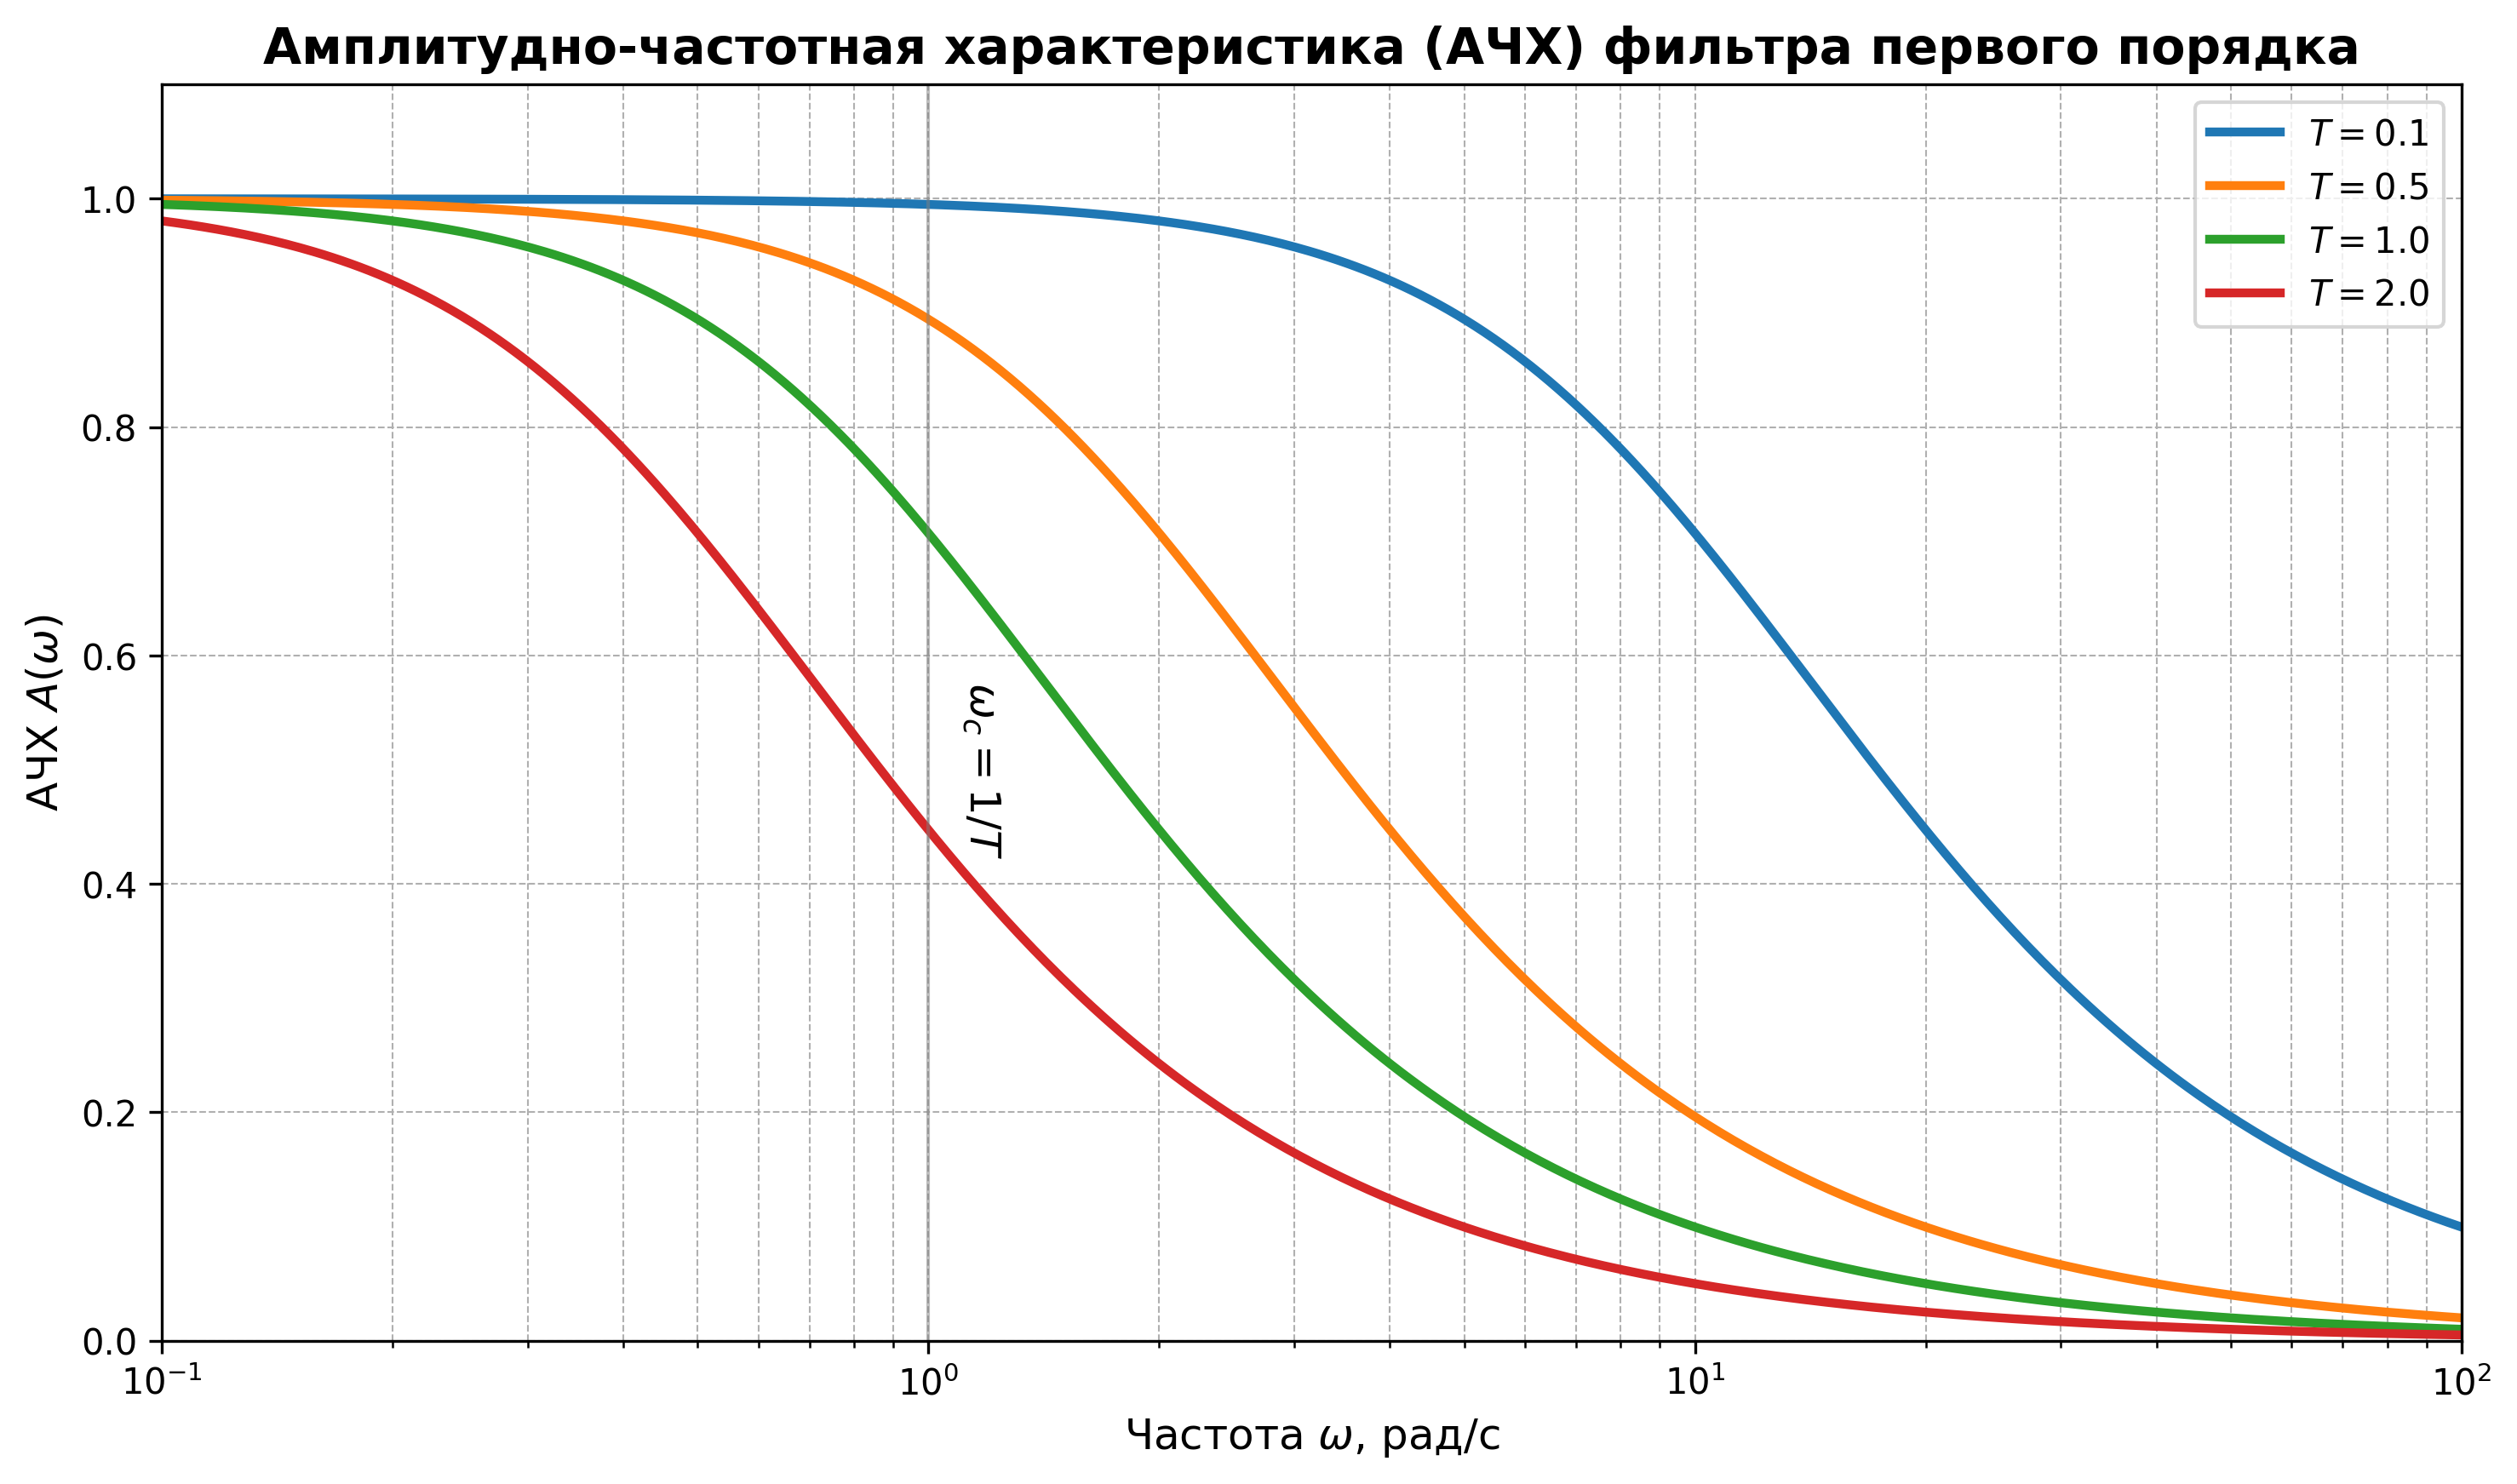
\includegraphics[width=0.85\textwidth]{images/bode_T.png}
    \caption{АЧХ фильтра первого порядка при различных значениях постоянной времени $T$}
    \label{fig:bode}
\end{figure}

\subsection{Эквивалентность методов фильтрации}
Динамическая фильтрация может быть реализована двумя способами:
\begin{enumerate}
    \item \textbf{Во временной области:} Решение дифференциального уравнения или вычисление свертки входного сигнала с весовой функцией $w(t)$ (обратным преобразованием Фурье от $W_1(i\omega)$). В коде это реализовано функцией \texttt{lsim}.
    \item \textbf{В частотной области:} Умножение спектра входного сигнала на частотную передаточную функцию $\hat{y}(\omega) = W_1(i\omega) \cdot \hat{u}(\omega)$ с последующим обратным преобразованием Фурье.
\end{enumerate}
Согласно теореме о свертке, эти методы должны давать идентичный результат. На рисунке~\ref{fig:methods_comparison} показано, что сигналы, полученные обоими способами, полностью совпадают. На рисунке~\ref{fig:spectrum_product} подтверждается, что модуль спектра отфильтрованного сигнала равен модулю произведения $W_1(i\omega) \cdot \hat{u}(\omega)$.

\begin{figure}[H]
    \centering
    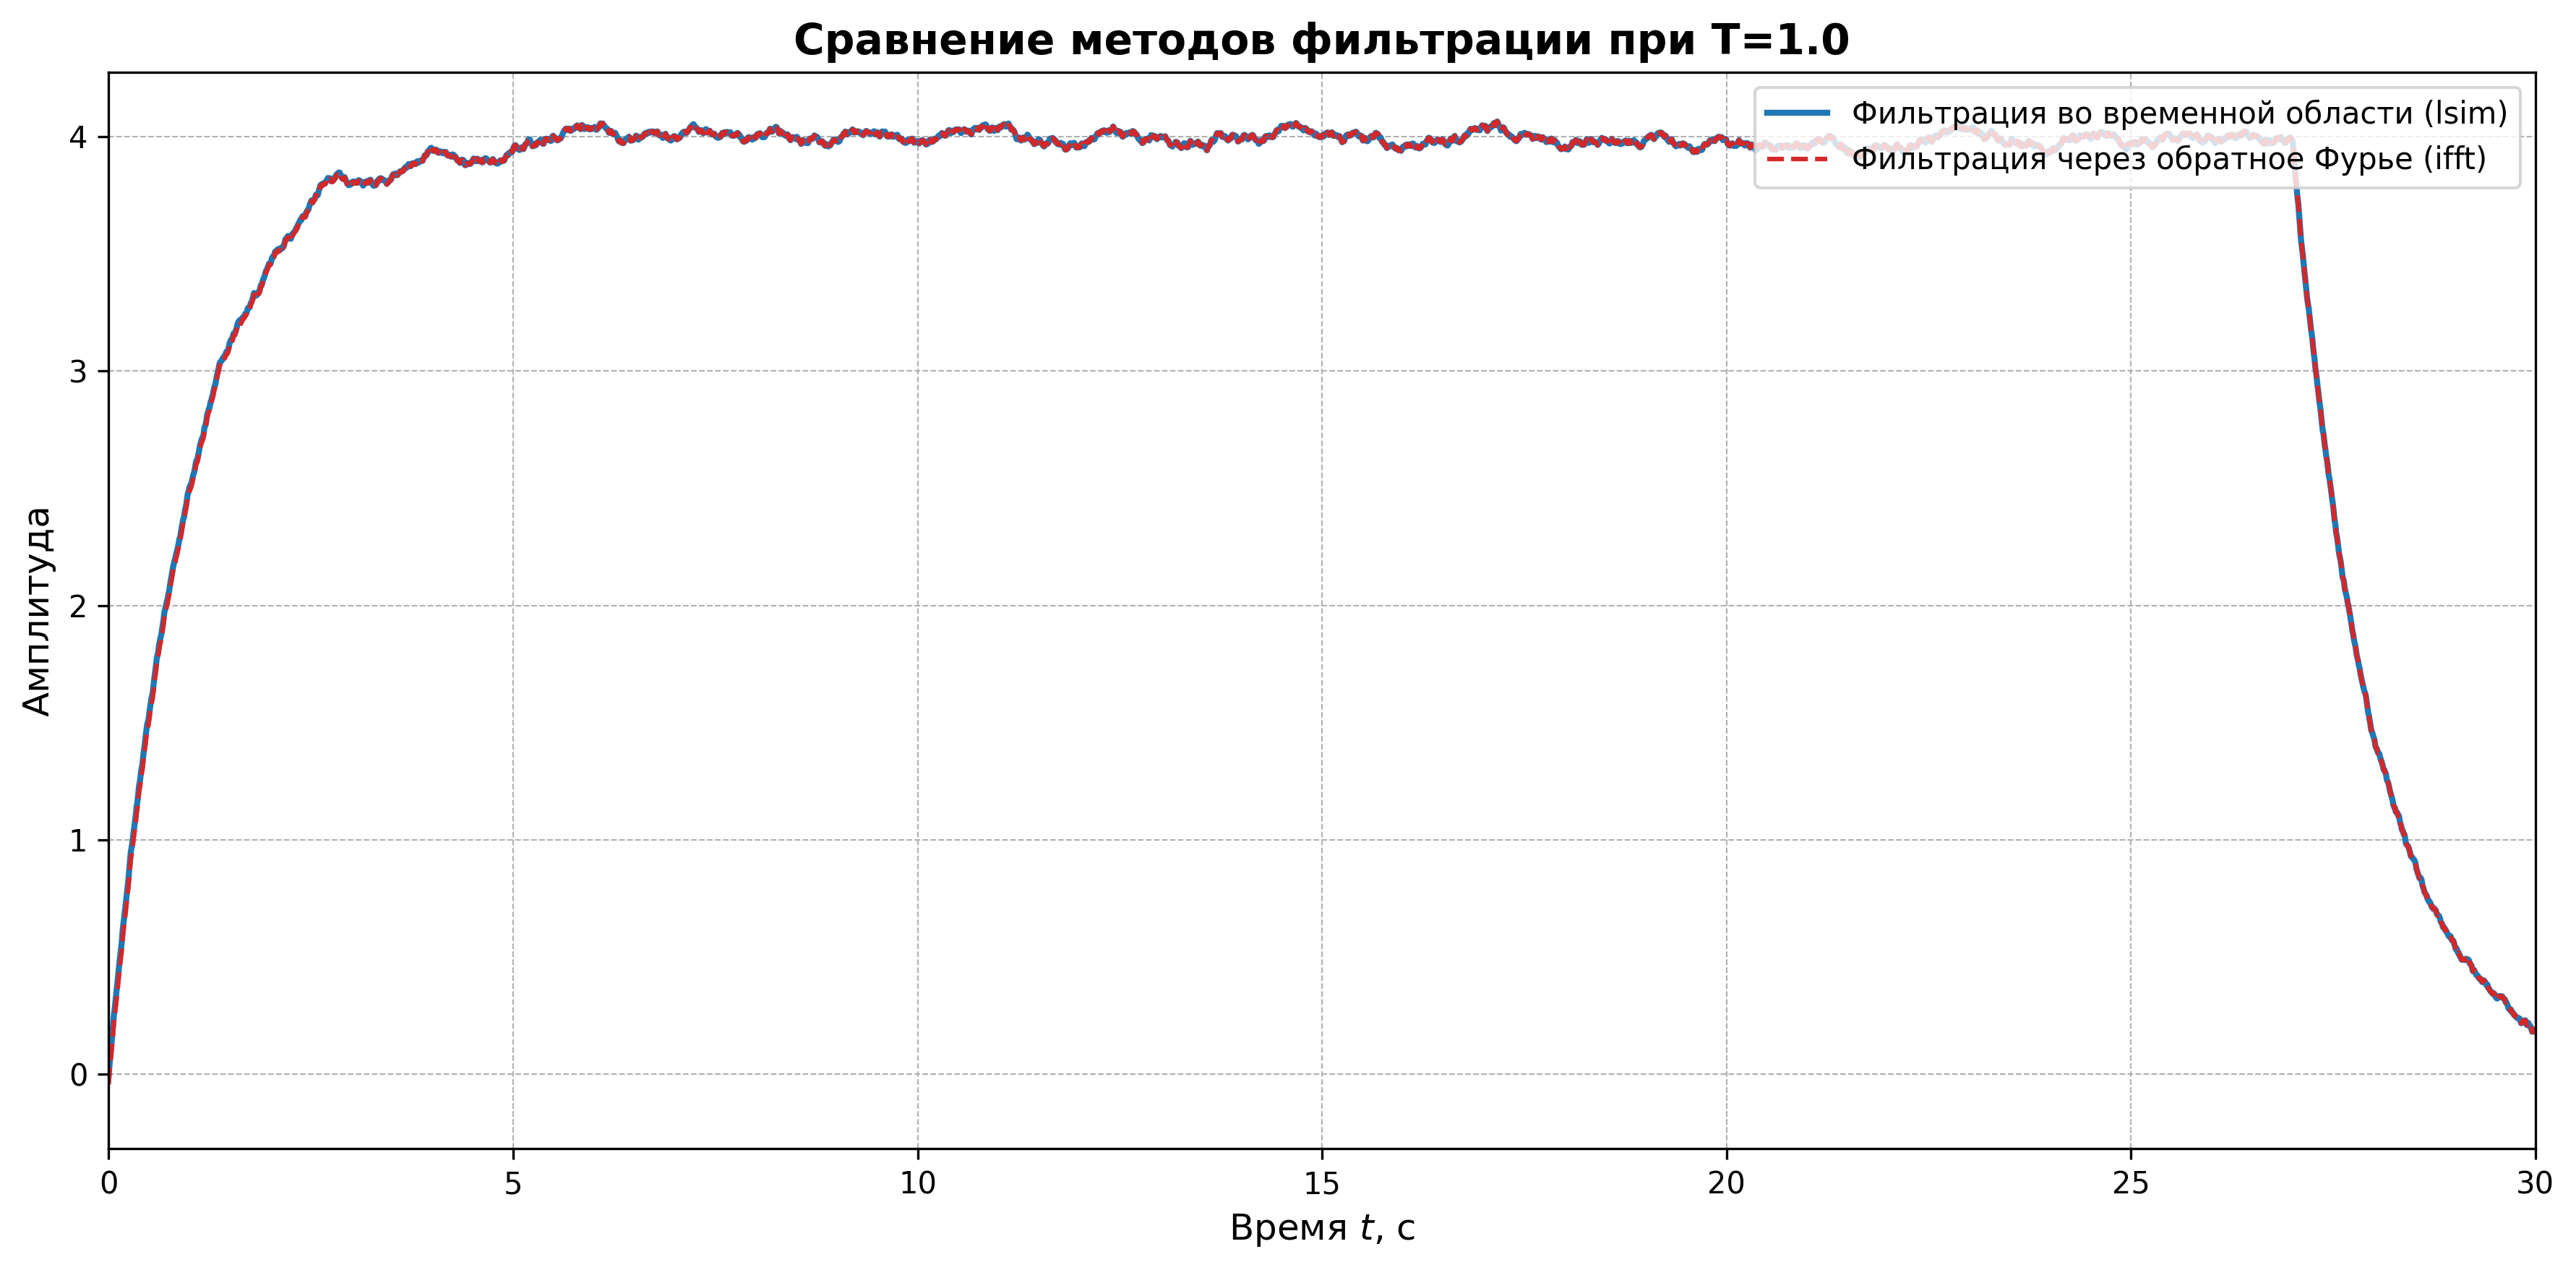
\includegraphics[width=0.85\textwidth]{images/filter_methods_comparison.png}
    \caption{Сравнение результатов фильтрации во временной области (lsim) и через обратное преобразование Фурье}
    \label{fig:methods_comparison}
\end{figure}

\begin{figure}[H]
    \centering
    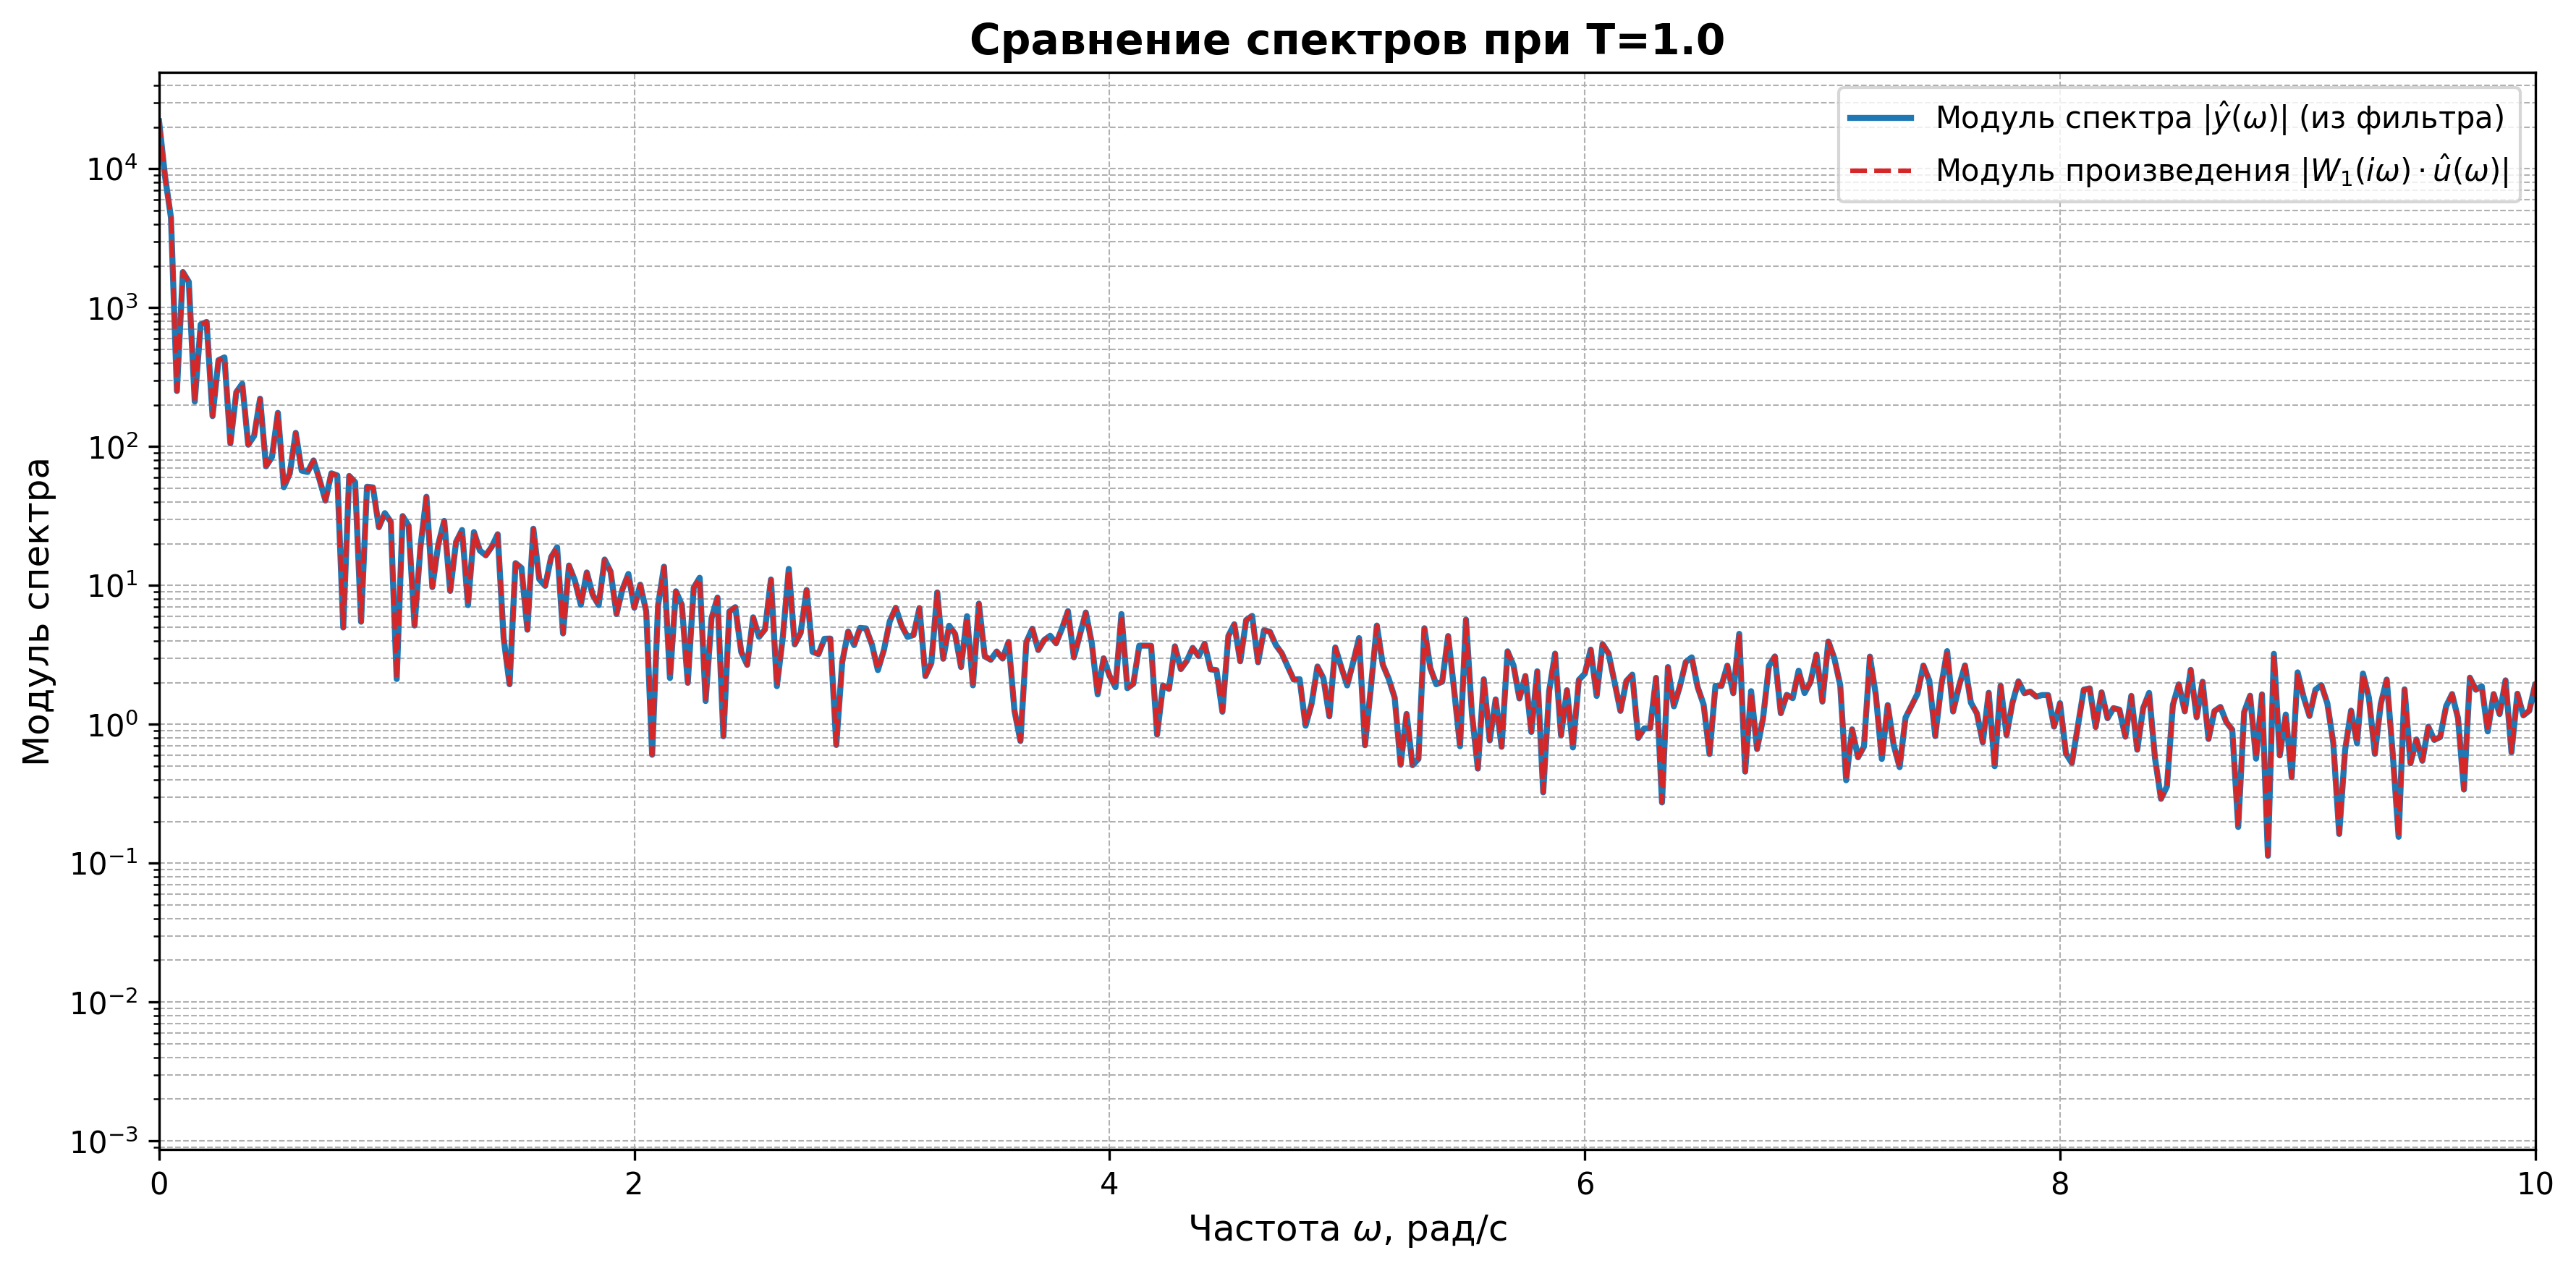
\includegraphics[width=0.85\textwidth]{images/spectrum_product_comparison.png}
    \caption{Сравнение модуля Фурье-образа фильтрованного сигнала и произведения $W_1(i\omega) \cdot \hat{u}(\omega)$}
    \label{fig:spectrum_product}
\end{figure}

\subsection{Исследование влияния параметров}
Качество восстановления сигнала зависит от постоянной времени $T$ и отношения сигнал/шум, определяемого амплитудой $a$.

\paragraph{Влияние постоянной времени $T$ при фиксированном $a$.}
На рисунке~\ref{fig:influence_T} показано влияние $T$ на результат фильтрации.
\begin{itemize}
    \item \textbf{Малое $T$ (например, $T=0.1$):} Фильтр имеет широкую полосу пропускания. Шум подавляется слабо, сигнал на выходе практически совпадает с зашумленным входом. Форма импульса сохраняется хорошо.
    \item \textbf{Оптимальное $T$ (например, $T=1.0$):} Наблюдается баланс. Высокочастотный шум эффективно подавляется, однако фронты импульса сглаживаются, амплитуда немного падает из-за фазового сдвига.
    \item \textbf{Большое $T$ (например, $T=2.0$):} Полоса пропускания очень узкая. Шум подавлен полностью, но полезный сигнал сильно искажен: импульс превращается в плавный "горб", теряя свою прямоугольную форму. Это неудачный случай, так как информация о фронтах потеряна.
\end{itemize}

\begin{figure}[H]
    \centering
    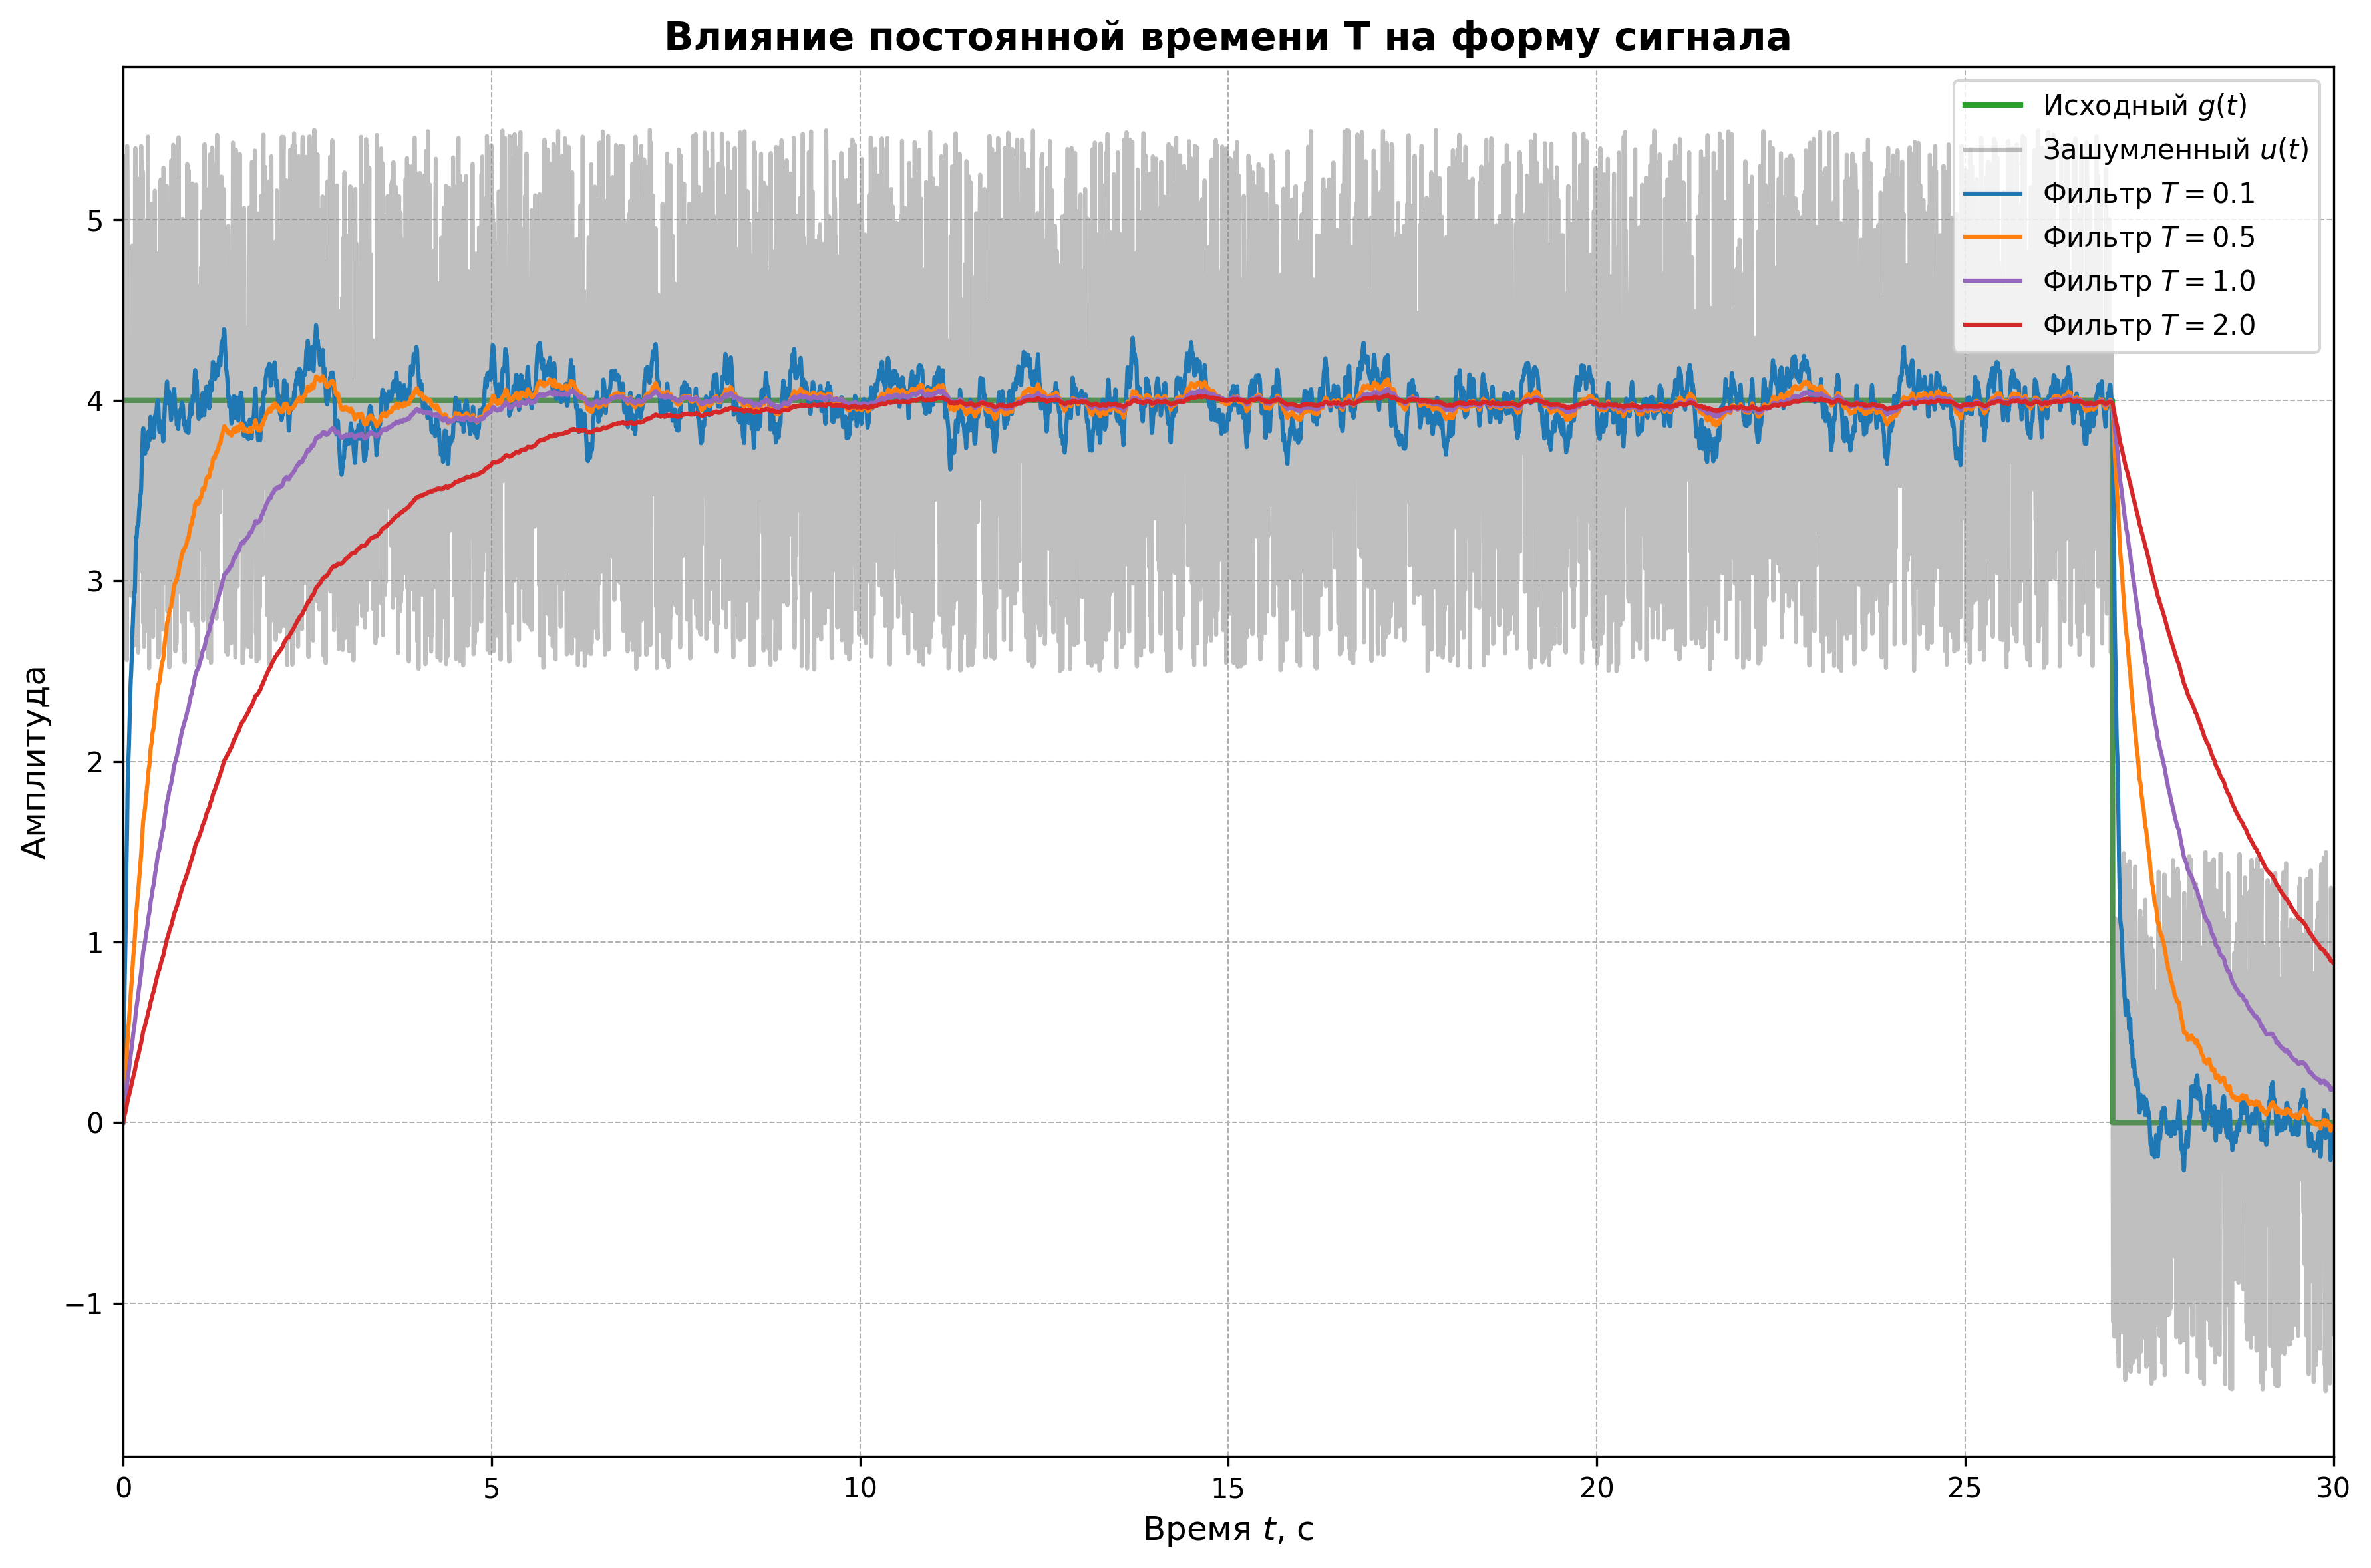
\includegraphics[width=0.85\textwidth]{images/influence_of_T.png}
    \caption{Влияние постоянной времени $T$ на форму сигнала при фиксированном $a$}
    \label{fig:influence_T}
\end{figure}

\paragraph{Влияние амплитуды $a$ при фиксированном $T$.}
На рисунке~\ref{fig:influence_a} показано, как меняется результат при изменении амплитуды сигнала (и, соответственно, отношения сигнал/шум) при фиксированном фильтре ($T=1.0$).
\begin{itemize}
    \item \textbf{Малое $a$ (например, $a=0.5$):} Полезный сигнал сопоставим по уровню с шумом. Даже после фильтрации остаточный шум маскирует полезную составляющую, восстановление формы невозможно.
    \item \textbf{Большое $a$ (например, $a=8.0$):} Отношение сигнал/шум высокое. Фильтр отлично справляется с задачей, форма импульса четко различима на фоне подавленного шума.
\end{itemize}
Таким образом, чем выше амплитуда полезного сигнала относительно шума, тем эффективнее работает динамическая фильтрация.

\begin{figure}[H]
    \centering
    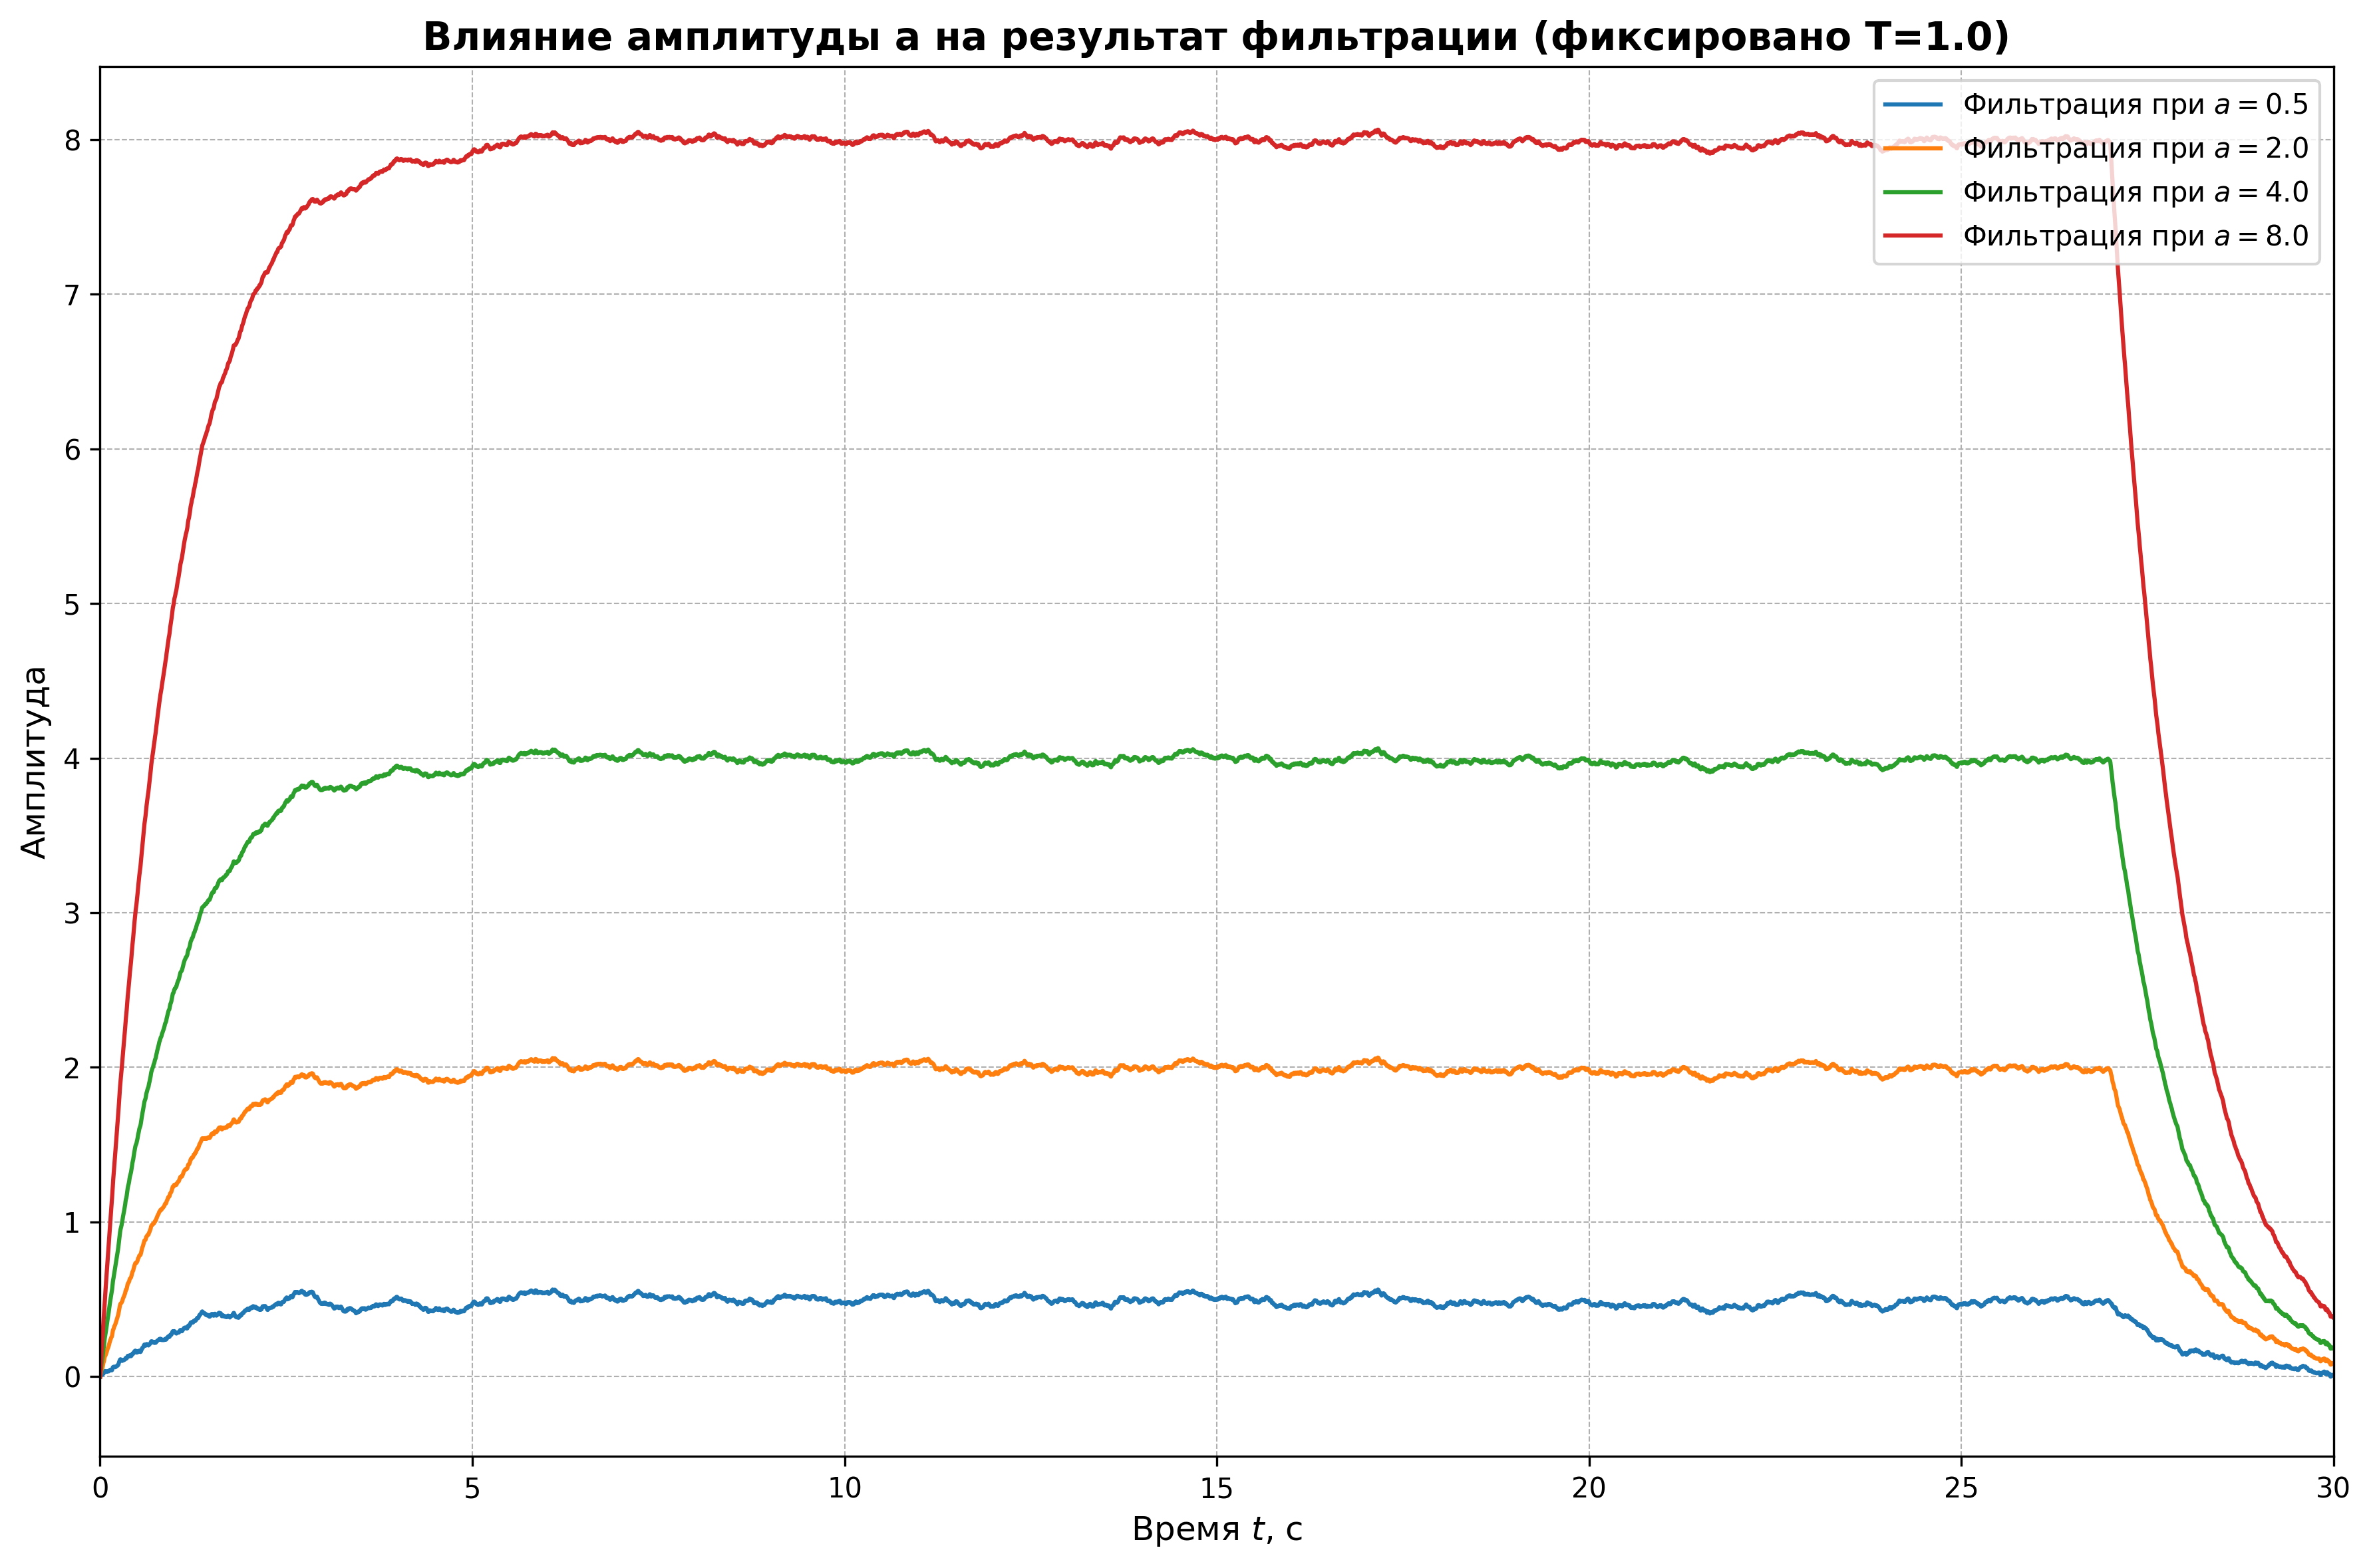
\includegraphics[width=0.85\textwidth]{images/influence_of_a.png}
    \caption{Влияние амплитуды $a$ на результат фильтрации при фиксированном $T=1.0$}
    \label{fig:influence_a}
\end{figure}

\subsection{Спектральный анализ}
На рисунках~\ref{fig:time_signals} и~\ref{fig:fft_modulus} представлены итоговые сравнительные графики исходного, зашумлённого и отфильтрованного сигналов во временной и частотной областях. В спектре зашумленного сигнала (синяя линия) видно, что на высоких частотах доминирует шум (ровная "полка"), в то время как спектр полезного сигнала (зеленая линия) затухает. Фильтр (пунктир) обрезает высокочастотную часть, оставляя основную энергию сигнала.

\begin{figure}[H]
    \centering
    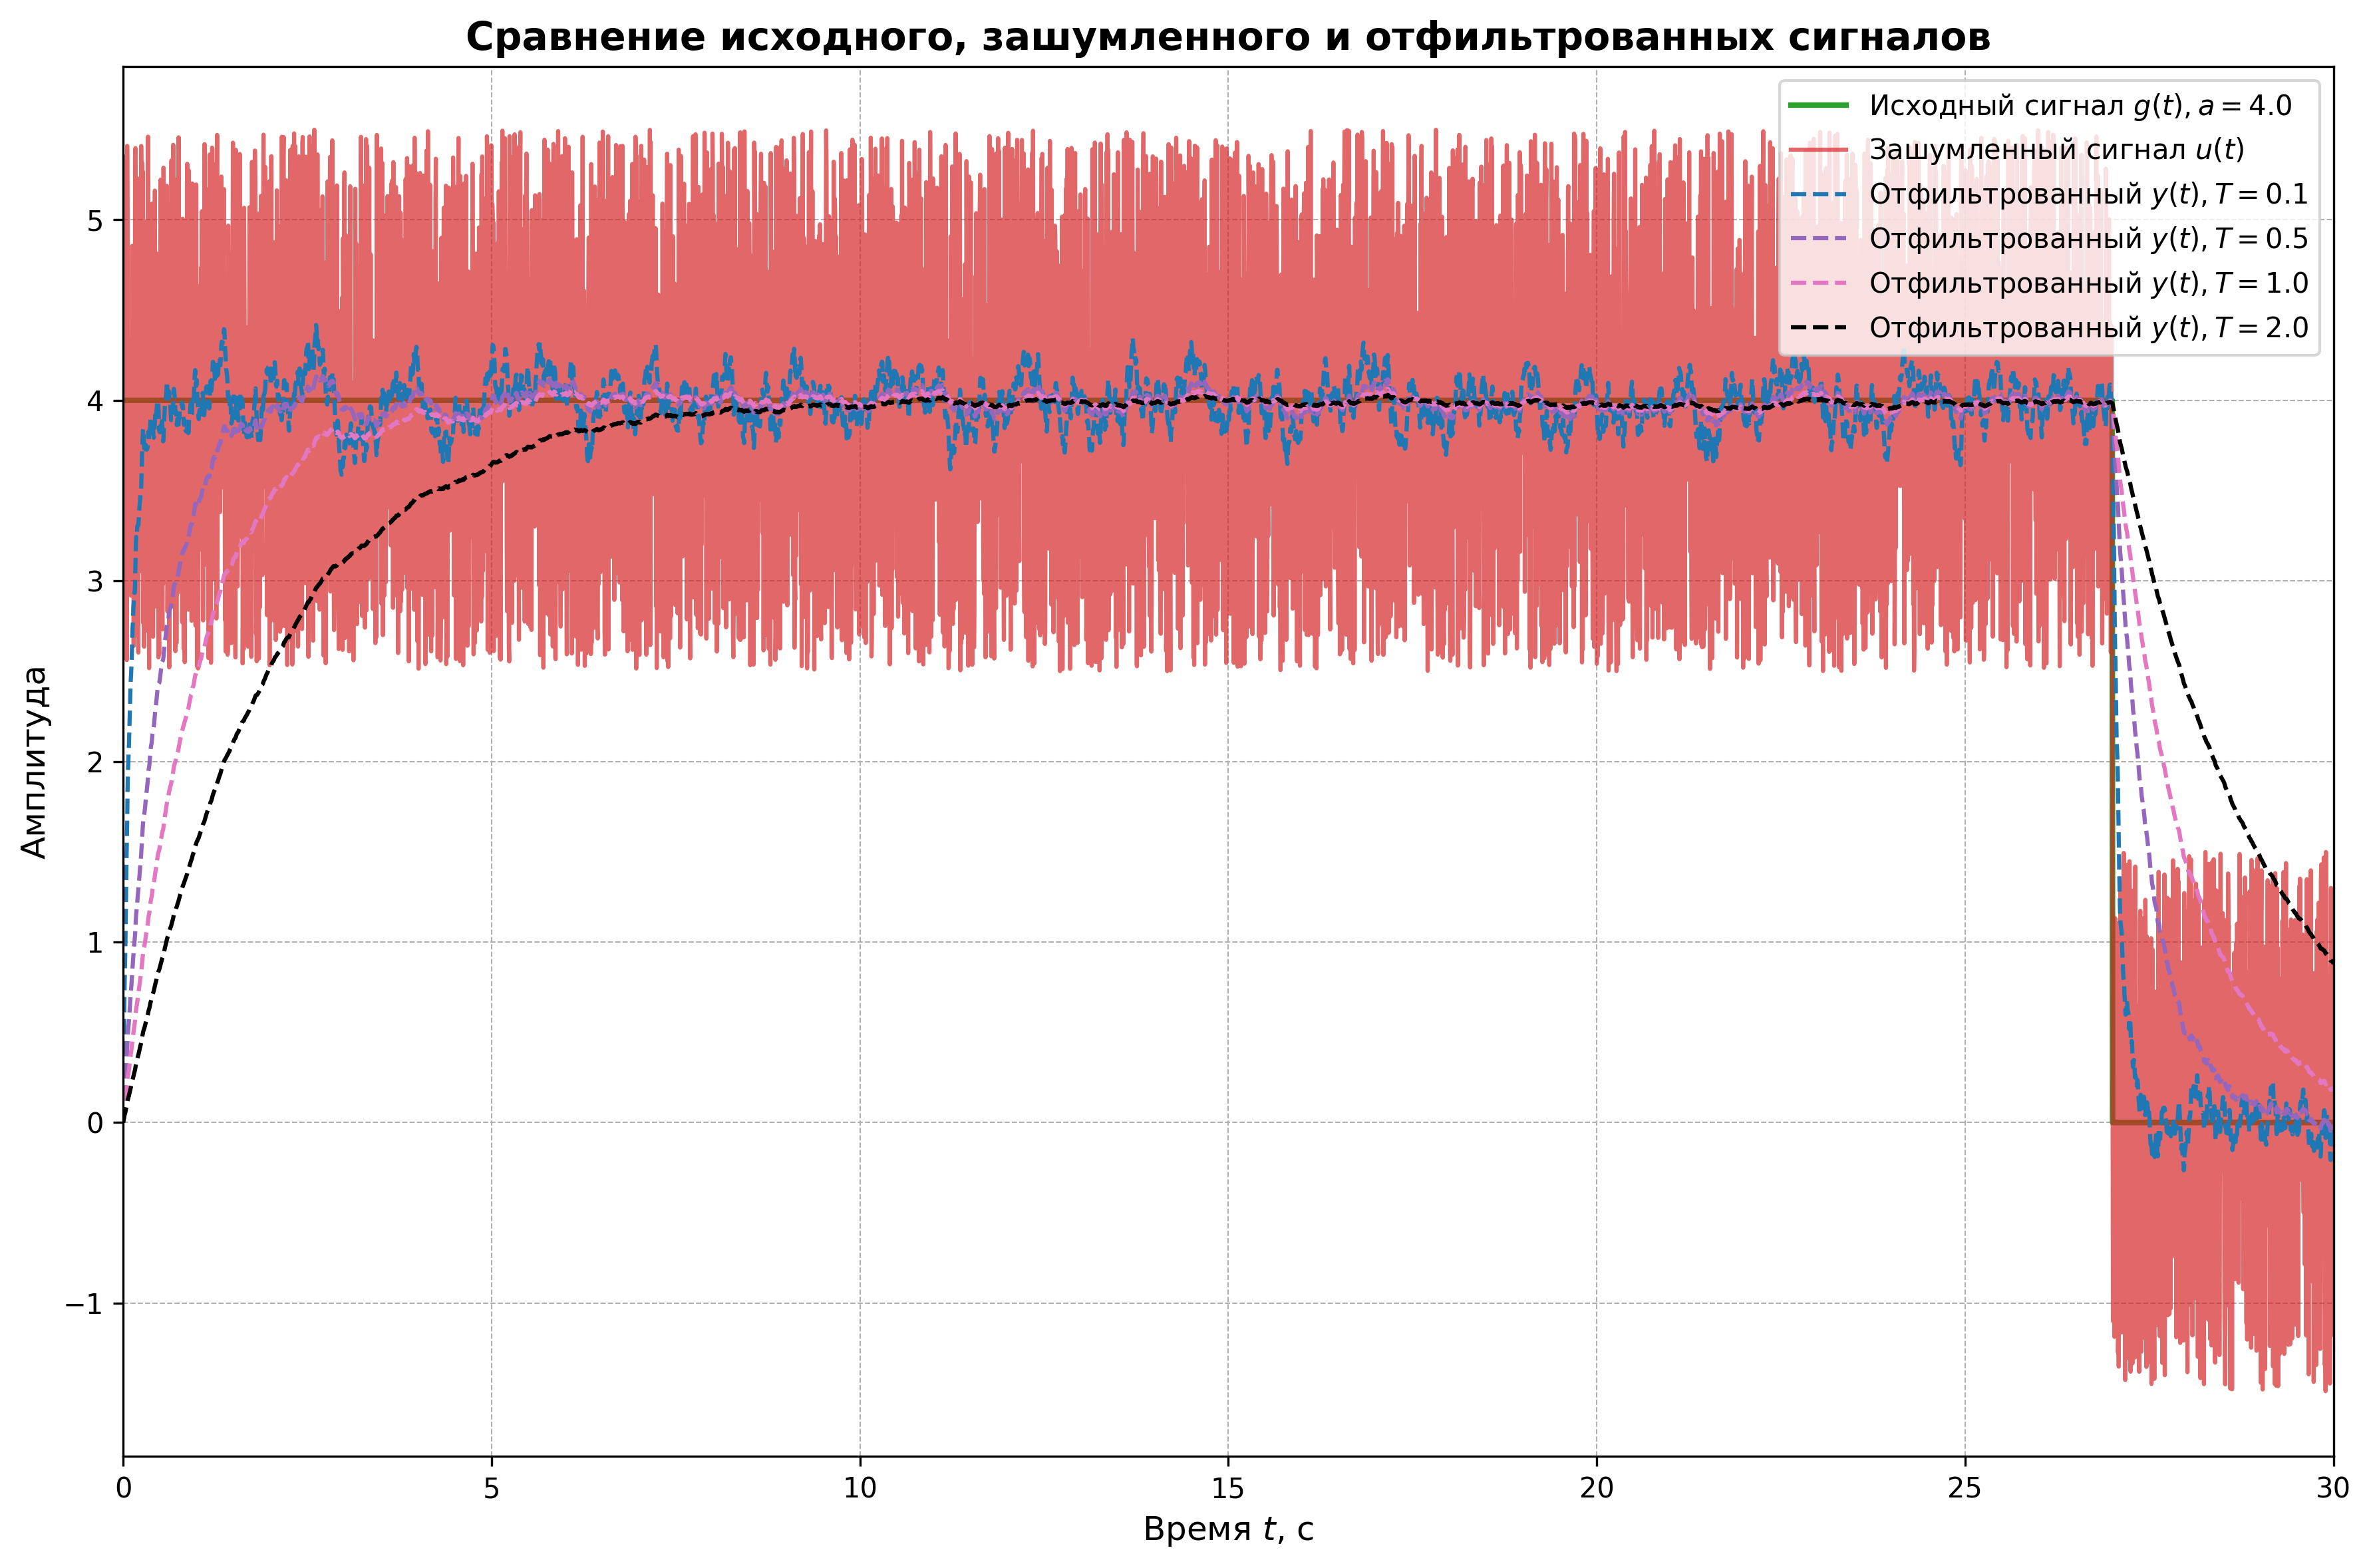
\includegraphics[width=0.85\textwidth]{images/time_signals.png}
    \caption{Сравнение исходного $g(t)$, зашумлённого $u(t)$ и фильтрованных сигналов при различных $T$}
    \label{fig:time_signals}
\end{figure}

\begin{figure}[H]
    \centering
    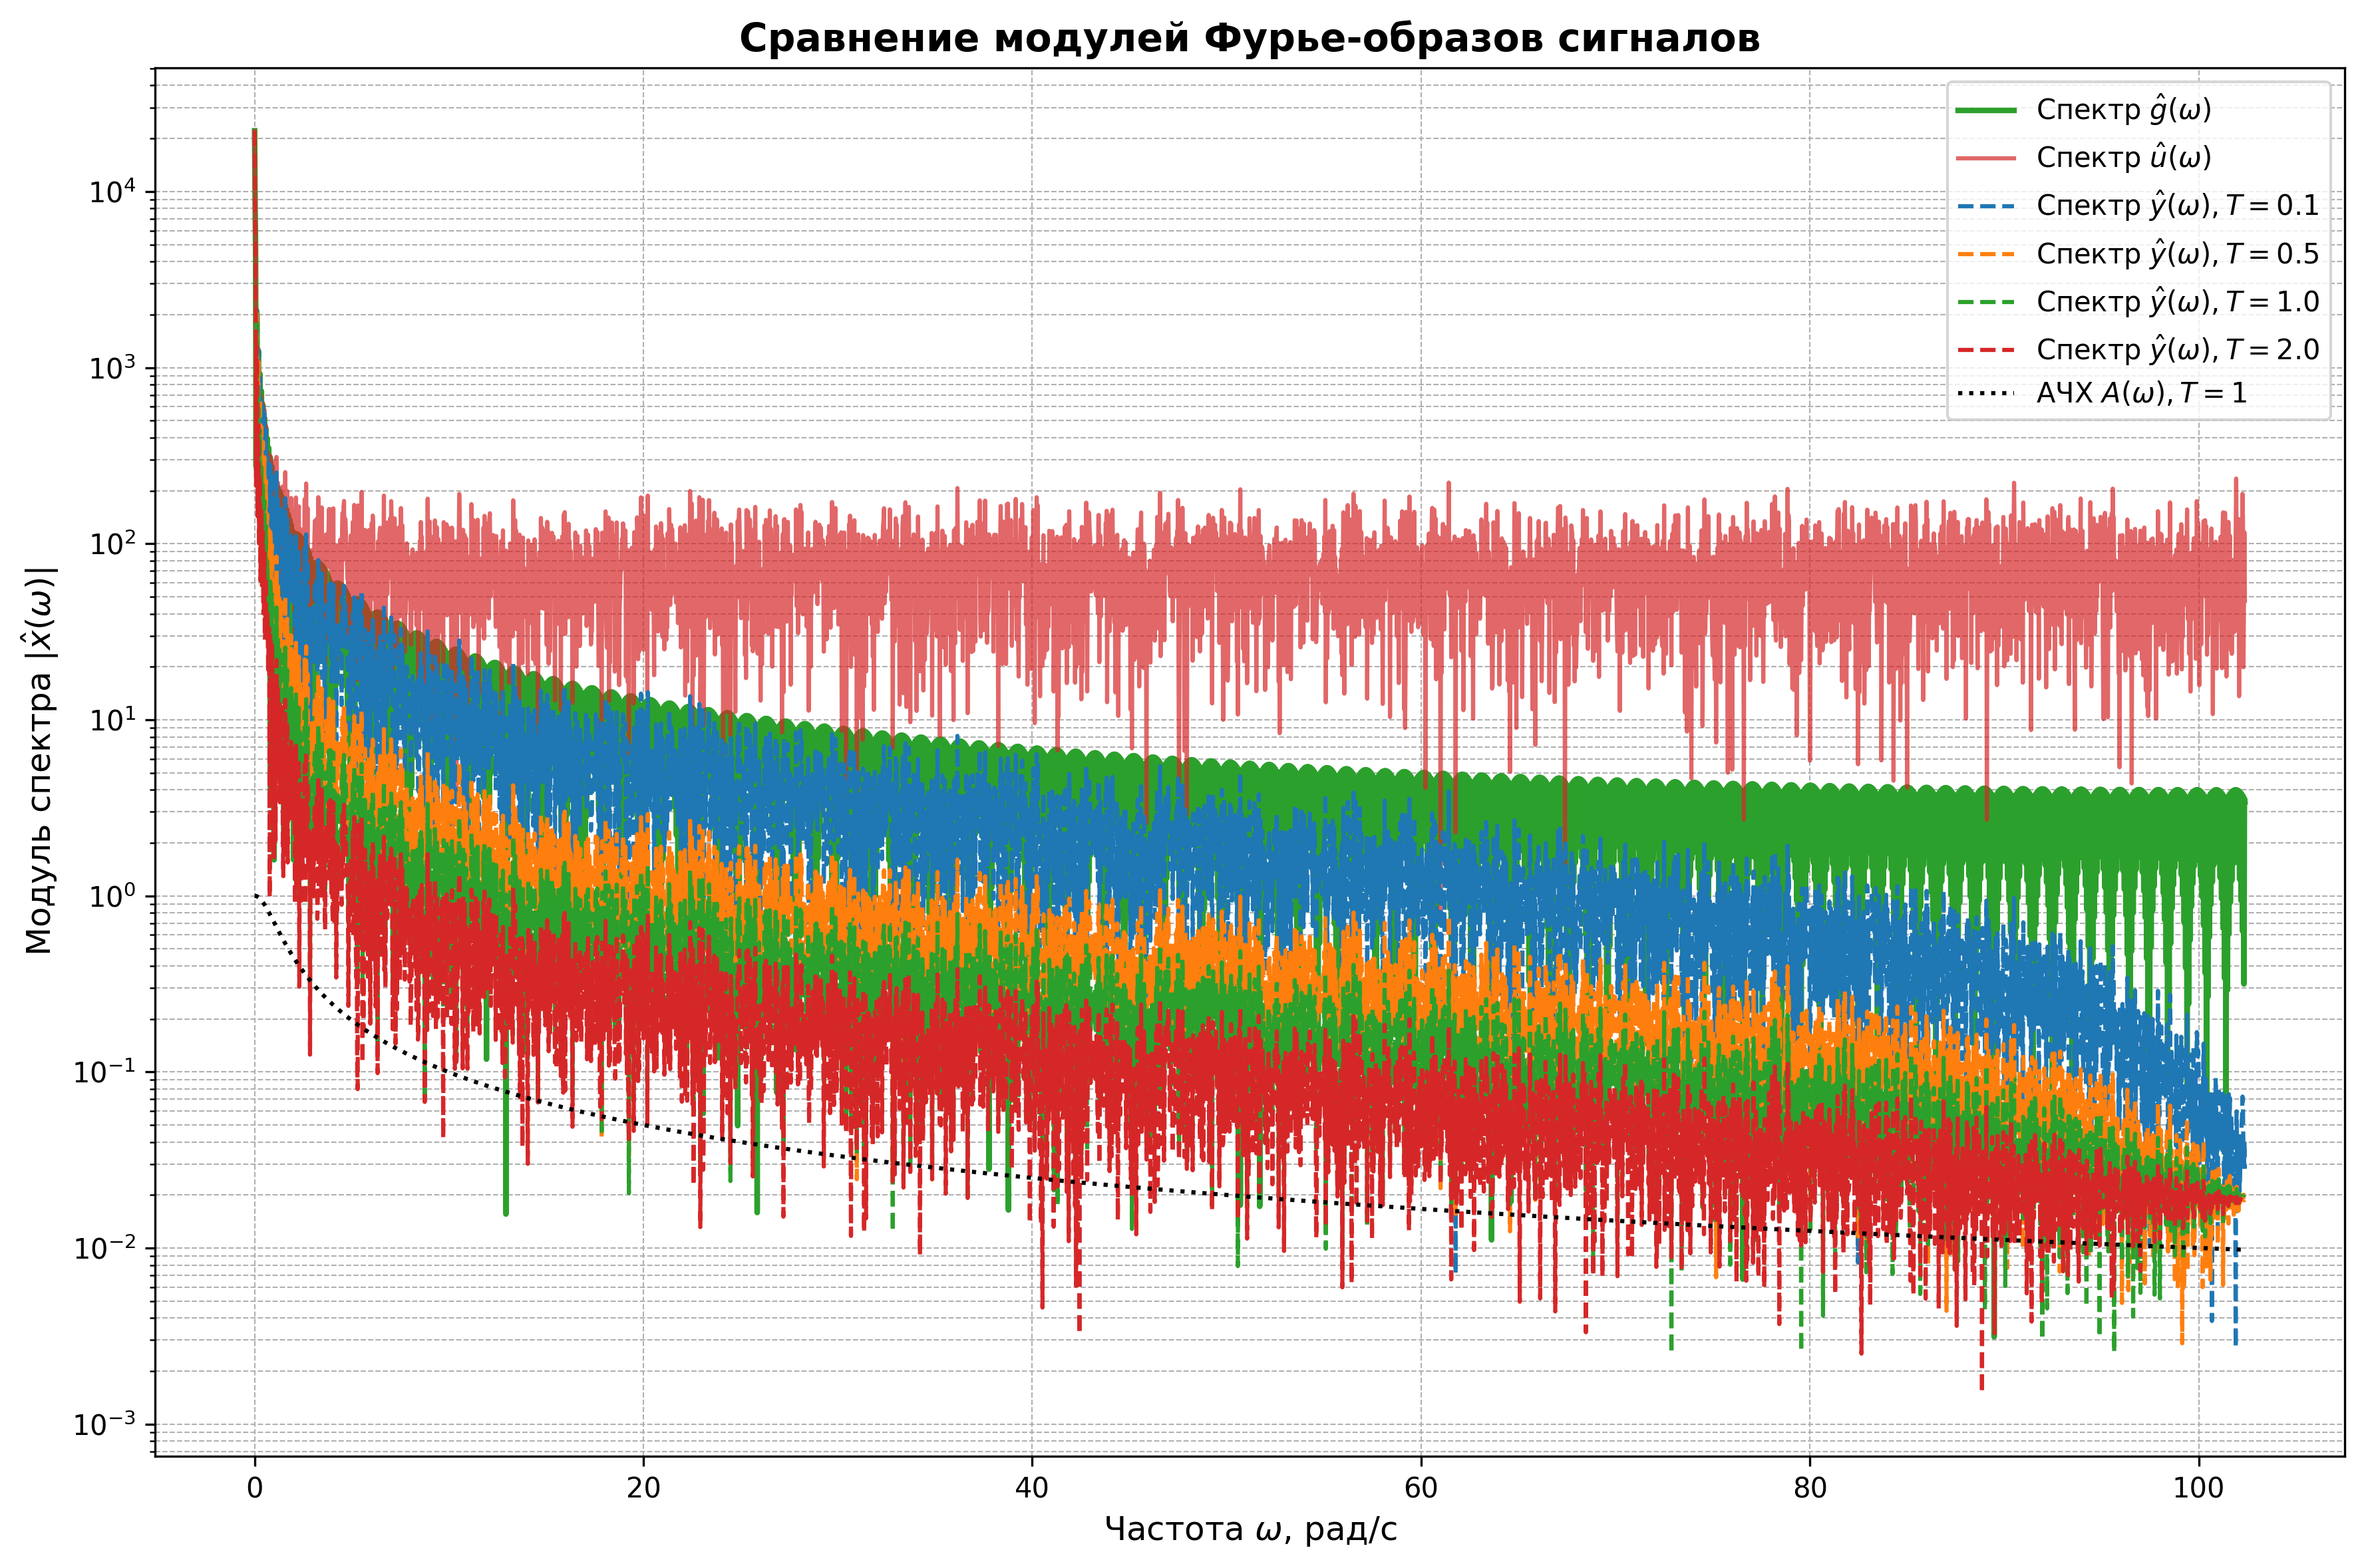
\includegraphics[width=0.85\textwidth]{images/fft_modulus.png}
    \caption{Сравнение модулей Фурье-образов $|\hat{g}(\omega)|$, $|\hat{u}(\omega)|$ и отфильтрованного сигнала}
    \label{fig:fft_modulus}
\end{figure}

\end{document}